\documentclass[9pt]{beamer}

% Beamer style
%\usetheme[secheader]{Madrid}
% \usetheme{CambridgeUS}
\useoutertheme{infolines}
\usecolortheme[rgb={0.65,0.15,0.25}]{structure}
% \usefonttheme[onlymath]{serif}
\beamertemplatenavigationsymbolsempty
%\AtBeginSubsection

% Packagesg
%\usepackage[french]{babel}
\usepackage[latin1]{inputenc}
\usepackage{color}
\usepackage{xspace}
\usepackage{enumerate}
\usepackage{dsfont, stmaryrd}
% \usepackage{amsmath, amsfonts, amssymb}
\usepackage{amsmath, amsfonts, amssymb, MnSymbol}
\usepackage{epsfig}
\usepackage{tikz}
\usepackage{url}
\usepackage{/home/robin/LATEX/Biblio/astats}
%\usepackage[all]{xy}
\usepackage{graphicx}

% Commands
% Maths
% \newtheorem{theorem}{Theorem}
% \newtheorem{definition}{Definition}
\newtheorem{proposition}{Proposition}
% \newtheorem{assumption}{Assumption}
% \newtheorem{algorithm}{Algorithm}
% \newtheorem{lemma}{Lemma}
% \newtheorem{remark}{Remark}
% \newtheorem{exercise}{Exercise}
% \newcommand{\propname}{Prop.}
% \newcommand{\proof}{\noindent{\sl Proof:}\quad}
% \newcommand{\eproof}{$\blacksquare$}

% \setcounter{secnumdepth}{3}
% \setcounter{tocdepth}{3}
\newcommand{\pref}[1]{\ref{#1} p.\pageref{#1}}
\newcommand{\qref}[1]{\eqref{#1} p.\pageref{#1}}

% Colors : http://latexcolor.com/
\definecolor{darkred}{rgb}{0.65,0.15,0.25}
\definecolor{darkgreen}{rgb}{0,0.4,0}
\definecolor{darkred}{rgb}{0.65,0.15,0.25}
\definecolor{amethyst}{rgb}{0.6, 0.4, 0.8}
\definecolor{asparagus}{rgb}{0.53, 0.66, 0.42}
\definecolor{applegreen}{rgb}{0.55, 0.71, 0.0}
\definecolor{awesome}{rgb}{1.0, 0.13, 0.32}
\definecolor{blue-green}{rgb}{0.0, 0.87, 0.87}
\definecolor{red-ggplot}{rgb}{0.52, 0.25, 0.23}
\definecolor{green-ggplot}{rgb}{0.42, 0.58, 0.00}
\definecolor{purple-ggplot}{rgb}{0.34, 0.21, 0.44}
\definecolor{blue-ggplot}{rgb}{0.00, 0.49, 0.51}

% Commands
\newcommand{\backupbegin}{
   \newcounter{finalframe}
   \setcounter{finalframe}{\value{framenumber}}
}
\newcommand{\backupend}{
   \setcounter{framenumber}{\value{finalframe}}
}
\newcommand{\emphase}[1]{\textcolor{darkred}{#1}}
\newcommand{\comment}[1]{\textcolor{gray}{#1}}
\newcommand{\paragraph}[1]{\textcolor{darkred}{#1}}
\newcommand{\refer}[1]{{\small{\textcolor{gray}{{\cite{#1}}}}}}
\newcommand{\Refer}[1]{{\small{\textcolor{gray}{{[#1]}}}}}
\newcommand{\goto}[1]{{\small{\textcolor{blue}{[\#\ref{#1}]}}}}
\renewcommand{\newblock}{}

\newcommand{\tabequation}[1]{{\medskip \centerline{#1} \medskip}}
% \renewcommand{\binom}[2]{{\left(\begin{array}{c} #1 \\ #2 \end{array}\right)}}

% Variables 
\newcommand{\Abf}{{\bf A}}
\newcommand{\Beta}{\text{B}}
\newcommand{\Bcal}{\mathcal{B}}
\newcommand{\Bias}{\xspace\mathbb B}
\newcommand{\Cor}{{\mathbb C}\text{or}}
\newcommand{\Cov}{{\mathbb C}\text{ov}}
\newcommand{\cl}{\text{\it c}\ell}
\newcommand{\Ccal}{\mathcal{C}}
\newcommand{\cst}{\text{cst}}
\newcommand{\Dcal}{\mathcal{D}}
\newcommand{\Ecal}{\mathcal{E}}
\newcommand{\Esp}{\xspace\mathbb E}
\newcommand{\Espt}{\widetilde{\Esp}}
\newcommand{\Covt}{\widetilde{\Cov}}
\newcommand{\Ibb}{\mathbb I}
\newcommand{\Fcal}{\mathcal{F}}
\newcommand{\Gcal}{\mathcal{G}}
\newcommand{\Gam}{\mathcal{G}\text{am}}
\newcommand{\Hcal}{\mathcal{H}}
\newcommand{\Jcal}{\mathcal{J}}
\newcommand{\Lcal}{\mathcal{L}}
\newcommand{\Mt}{\widetilde{M}}
\newcommand{\mt}{\widetilde{m}}
\newcommand{\Nbb}{\mathbb{N}}
\newcommand{\Mcal}{\mathcal{M}}
\newcommand{\Ncal}{\mathcal{N}}
\newcommand{\Ocal}{\mathcal{O}}
\newcommand{\pt}{\widetilde{p}}
\newcommand{\Pt}{\widetilde{P}}
\newcommand{\Pbb}{\mathbb{P}}
\newcommand{\Pcal}{\mathcal{P}}
\newcommand{\Qcal}{\mathcal{Q}}
\newcommand{\qt}{\widetilde{q}}
\newcommand{\Rbb}{\mathbb{R}}
\newcommand{\Sbb}{\mathbb{S}}
\newcommand{\Scal}{\mathcal{S}}
\newcommand{\st}{\widetilde{s}}
\newcommand{\St}{\widetilde{S}}
\newcommand{\Tcal}{\mathcal{T}}
\newcommand{\todo}{\textcolor{red}{TO DO}}
\newcommand{\Ucal}{\mathcal{U}}
\newcommand{\Un}{\math{1}}
\newcommand{\Vcal}{\mathcal{V}}
\newcommand{\Var}{\mathbb V}
\newcommand{\Vart}{\widetilde{\Var}}
\newcommand{\Zcal}{\mathcal{Z}}

% Symboles & notations
\newcommand\independent{\protect\mathpalette{\protect\independenT}{\perp}}\def\independenT#1#2{\mathrel{\rlap{$#1#2$}\mkern2mu{#1#2}}} 
\renewcommand{\d}{\text{\xspace d}}
\newcommand{\gv}{\mid}
\newcommand{\ggv}{\, \| \, }
% \newcommand{\diag}{\text{diag}}
\newcommand{\card}[1]{\text{card}\left(#1\right)}
\newcommand{\trace}[1]{\text{tr}\left(#1\right)}
\newcommand{\matr}[1]{\boldsymbol{#1}}
\newcommand{\matrbf}[1]{\mathbf{#1}}
\newcommand{\vect}[1]{\matr{#1}} %% un peu inutile
\newcommand{\vectbf}[1]{\matrbf{#1}} %% un peu inutile
\newcommand{\trans}{\intercal}
\newcommand{\transpose}[1]{\matr{#1}^\trans}
\newcommand{\crossprod}[2]{\transpose{#1} \matr{#2}}
\newcommand{\tcrossprod}[2]{\matr{#1} \transpose{#2}}
\newcommand{\matprod}[2]{\matr{#1} \matr{#2}}
\DeclareMathOperator*{\argmin}{arg\,min}
\DeclareMathOperator*{\argmax}{arg\,max}
\DeclareMathOperator{\sign}{sign}
\DeclareMathOperator{\tr}{tr}
\newcommand{\ra}{\emphase{$\rightarrow$} \xspace}

% Hadamard, Kronecker and vec operators
\DeclareMathOperator{\Diag}{Diag} % matrix diagonal
\DeclareMathOperator{\diag}{diag} % vector diagonal
\DeclareMathOperator{\mtov}{vec} % matrix to vector
\newcommand{\kro}{\otimes} % Kronecker product
\newcommand{\had}{\odot}   % Hadamard product

% TikZ
\newcommand{\nodesize}{2em}
\newcommand{\edgeunit}{2.5*\nodesize}
\newcommand{\edgewidth}{1pt}
\tikzstyle{node}=[draw, circle, fill=black, minimum width=.75\nodesize, inner sep=0]
\tikzstyle{square}=[rectangle, draw]
\tikzstyle{param}=[draw, rectangle, fill=gray!50, minimum width=\nodesize, minimum height=\nodesize, inner sep=0]
\tikzstyle{hidden}=[draw, circle, fill=gray!50, minimum width=\nodesize, inner sep=0]
\tikzstyle{hiddenred}=[draw, circle, color=red, fill=gray!50, minimum width=\nodesize, inner sep=0]
\tikzstyle{observed}=[draw, circle, minimum width=\nodesize, inner sep=0]
\tikzstyle{observedred}=[draw, circle, minimum width=\nodesize, color=red, inner sep=0]
\tikzstyle{eliminated}=[draw, circle, minimum width=\nodesize, color=gray!50, inner sep=0]
\tikzstyle{empty}=[draw, circle, minimum width=\nodesize, color=white, inner sep=0]
\tikzstyle{blank}=[color=white]
\tikzstyle{nocircle}=[minimum width=\nodesize, inner sep=0]

\tikzstyle{edge}=[-, line width=\edgewidth]
\tikzstyle{edgebendleft}=[-, >=latex, line width=\edgewidth, bend left]
\tikzstyle{edgebendright}=[-, >=latex, line width=\edgewidth, bend right]
\tikzstyle{lightedge}=[-, line width=\edgewidth, color=gray!50]
\tikzstyle{lightedgebendleft}=[-, >=latex, line width=\edgewidth, bend left, color=gray!50]
\tikzstyle{lightedgebendright}=[-, >=latex, line width=\edgewidth, bend right, color=gray!50]
\tikzstyle{edgered}=[-, line width=\edgewidth, color=red]
\tikzstyle{edgebendleftred}=[-, >=latex, line width=\edgewidth, bend left, color=red]
\tikzstyle{edgebendrightred}=[-, >=latex, line width=\edgewidth, bend right, color=red]

\tikzstyle{arrow}=[->, >=latex, line width=\edgewidth]
\tikzstyle{arrowbendleft}=[->, >=latex, line width=\edgewidth, bend left]
\tikzstyle{arrowbendright}=[->, >=latex, line width=\edgewidth, bend right]
\tikzstyle{arrowred}=[->, >=latex, line width=\edgewidth, color=red]
\tikzstyle{arrowbendleftred}=[->, >=latex, line width=\edgewidth, bend left, color=red]
\tikzstyle{arrowbendrightred}=[->, >=latex, line width=\edgewidth, bend right, color=red]
\tikzstyle{arrowblue}=[->, >=latex, line width=\edgewidth, color=blue]
\tikzstyle{dashedarrow}=[->, >=latex, dashed, line width=\edgewidth]
\tikzstyle{dashededge}=[-, >=latex, dashed, line width=\edgewidth]
\tikzstyle{dashededgebendleft}=[-, >=latex, dashed, line width=\edgewidth, bend left]
\tikzstyle{lightarrow}=[->, >=latex, line width=\edgewidth, color=gray!50]


% Directory
\newcommand{\fignet}{/home/robin/RECHERCHE/RESEAUX/EXPOSES/FIGURES}
\newcommand{\figtree}{/home/robin/RECHERCHE/BAYES/VBEM-IS/VBEM-IS.git/Data/Tree/Fig}
\newcommand{\figbayes}{/home/robin/RECHERCHE/BAYES/EXPOSES/FIGURES}
\newcommand{\figzebra}{/home/robin/RECHERCHE/BAYES/VBEM-IS/VBEM-IS.git/Data/Zebra/Fig}
\newcommand{\figeco}{/home/robin/RECHERCHE/ECOLOGIE/EXPOSES/FIGURES}

%====================================================================
%====================================================================

%====================================================================
%====================================================================
\begin{document}
%====================================================================
%====================================================================

%====================================================================
\title[Improving variational inference]{Improving the variational inference of latent variable models in ecology}

\author[S. Robin]{S. Robin \\ ~\\
    Joint work with S. Donnet and J. Stoehr
  }

\institute[]{\small Sorbonne universit\'e \\ 
Laboratoire de Probabilit\'es, Statistique et Mod\'elisation (LPSM) \\ ~ \\ ~}

\date[Feb.'25, UVSQ]{
Mod\'elisation, analyse statistique, et applications en \'ecologie et climatologie}

%====================================================================
%====================================================================
\maketitle
%====================================================================

%====================================================================
%====================================================================
\section{Latent variable models in ecology}
\frame{\frametitle{Outline} \tableofcontents[currentsection]}
%====================================================================
\frame{\frametitle{Latent variable models in ecology}

  \paragraph{Latent  ('hidden', 'unobserved', ...) variables} are widely used in statistical ecology  \refer{PeG22b} to 
  \begin{itemize}
    \setlength{\itemsep}{.5\baselineskip}
    \item account for heterogeneity (species clustering, over-dispersion or 'excess' of zeros in population sizes), 
    \item encode dependency (due to space, genetics, ...), 
    \item represent a 'true' signal, observed with noise (animal movement), 
    \item ...
  \end{itemize}

  \bigskip \bigskip 
  \paragraph{Statistical perspective.} 
  \begin{itemize}
    \setlength{\itemsep}{.5\baselineskip}
    \item Number of latent variables $\simeq$ number of observed variable.
    \item The inference of the mode parameters would be much easier if they were observed.
  \end{itemize}

}

%====================================================================
\frame{\frametitle{Joint species distribution models}

  \paragraph{Aim.} 
  Describe/understand the relationships that living species share with each other and with their environment (biogeography, community ecology). 

  \bigskip \bigskip \pause 
  \paragraph{Species distribution models.} 
  $n$ sites, $x_i =$ vector of environmental descriptors for site $i$, $Y_i =$ number of individual from the species of interest observed in site $i$:
  $$
  Y_i \sim \Fcal(\cdot; x_i, \beta).
  $$
  $\to$ Generalized linear (mixed) model \refer{ElL09,ZIW09}

  \bigskip \bigskip \pause
  \paragraph{Joint species distribution models.} 
  Same, but $Y_i = (Y_{i1}, \dots Y_{ip}) =$ vector of counts for $p$ species of interest observed in site $i$:
  $$
  Y_i \sim \Fcal_p(\cdot; x_i, \beta, \Sigma)
  $$
  $\to$ Multivariate generalized linear mixed model  \refer{WBO15,OvA20}
  
}

%====================================================================
\frame{\frametitle{Poisson log-normal model}

  \paragraph{A joint species distribution model:} 
  Poisson-log normal distribution \refer{AiH89,CMR21}
  \begin{align*}
    & \text{in each site $i = 1 \dots n$:} & 
    Z_i & \sim \Ncal_p(0, \emphase{\Sigma}) \\
    & \text{for each specie $j = 1 \dots p$:} &
    Y_{ij} \mid Z_{ij} & \sim \Pcal_p(\exp(x_i^\top \emphase{\beta_j} + Z_{ij}))
  \end{align*} \pause
  \begin{itemize}
    \item $\beta_j =$ effects of the environmental covariates on species $j$ (\emphase{\sl abiotic} interactions)
    \item $\Sigma =$ between-species covariance matrix  (\emphase{\sl biotic} interactions)
  \end{itemize}

  \bigskip \bigskip \pause
  \paragraph{Fish species from the Barents sea.} 
  $n = 89$, $p = 30$, $d = 4$ covariates
  $$
  \begin{tabular}{ccc}
    Covariate effects & 
    Covariate induced & 
    Between species \\
    $\widehat{B}$ & 
    correlation & 
    correlation  $\widehat{\Sigma}$ \\
    \includegraphics[width=.25\textwidth, trim=20 20 50 20, clip=]{\figeco/BarentsFish-coeffAll-woIntercept} & 
    \includegraphics[width=.25\textwidth, trim=20 20 50 20, clip=]{\figeco/BarentsFish-corrPred} & 
    \includegraphics[width=.25\textwidth, trim=20 20 50 20, clip=]{\figeco/BarentsFish-corrAll}
  \end{tabular}
  $$
}

%====================================================================
\frame{\frametitle{Species interaction networks}

  \paragraph{Aim.} 
  Understand the organization of species interactions, viewed as a network:
  \begin{itemize}
    \item trophic (who-eats-who; unipartite, directed), 
    \item plant-pollinator, host-parasites (bipartite), 
    \item number of shared parasites (unipartite, un-oriented, weighted), 
    \item ....
  \end{itemize}

  \bigskip \bigskip \pause
  \paragraph{Network model.} $n$ species, $x_i =$ vector of covariates for species $i$, $x_{ij}$ vector of covariates for the pair of species $(i, j)$, $Y_{ij} =$ interaction between species $i$ and $j$:
  $$
  Y = (Y_{ij})_{1 \leq i, j, \leq n} \sim \Fcal(\cdot; (x_i)_{1 \leq i \leq n}, (x_{ij})_{1 \leq i, j \leq n}, \theta).
  $$
  $\to$ Exponential random graph models (ERGM: \refer{HHB08}), Block-models \refer{HoL79,GoN03} (review: \refer{MaR14})
  
}

%====================================================================
\frame{\frametitle{Stochastic block-model (1/2)}

  \paragraph{A network model:} Stochastic block-model with covariates \refer{MRV10}
  \begin{align*}
    & \text{for each species $i = 1 \dots n$:} & 
    Z_i & \sim \Mcal_p(0, \emphase{\pi}) \\
    & \text{for each pair of species $(i, j) \in \{1 \dots n\}$:} &
    Y_{ij} \mid Z_i = q, Z_j = \ell & \sim \Pcal(\exp(\alpha_{q\ell} + x_{ij}^\top \emphase{\beta}))
  \end{align*} \pause
  \begin{itemize}
    \item $\pi_q =$ proportion of species belonging to group $k$ (\emphase{\sl node clustering})
    \item $\beta =$ effect of the covariates on the interaction intensity
  \end{itemize}
  
  \bigskip \bigskip \pause
  \paragraph{Tree interactions.} 
  $n = 51$ species, $Y_{ij} =$ number of common fungal parasites \refer{VPD08}
  $$
  \begin{tabular}{ccc}
    Observed network &  & Observed adjacency matrix \\
    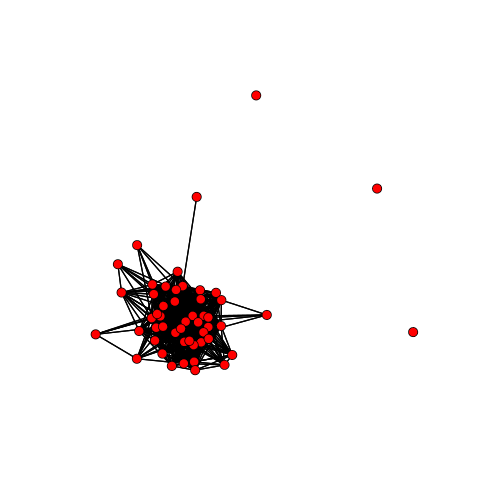
\includegraphics[width=.25\textwidth, trim=0 0 50 20, clip=]{\figbayes/FigUVSQ-Tree-Network} & 
    \qquad \qquad & 
    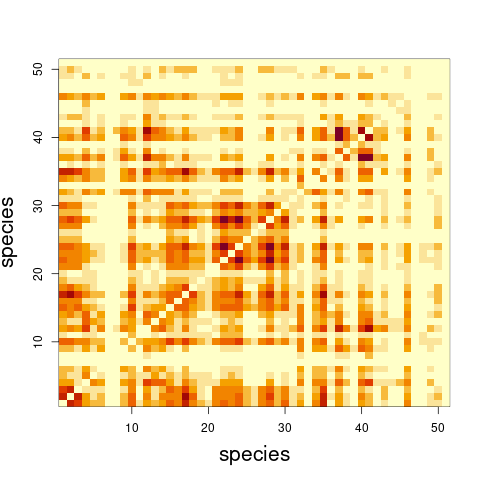
\includegraphics[width=.25\textwidth, trim=0 10 50 20, clip=]{\figbayes/FigUVSQ-Tree-Adjacency}
  \end{tabular}
  $$
}
  
%====================================================================
\frame{\frametitle{Stochastic block-model (2/2)}

  \paragraph{Tree interactions.} 
  $d = 3$ edge covariates (distances)
  $$
  \begin{tabular}{ccc}
    Genetic (log) & Geographic & Taxonomic \\
    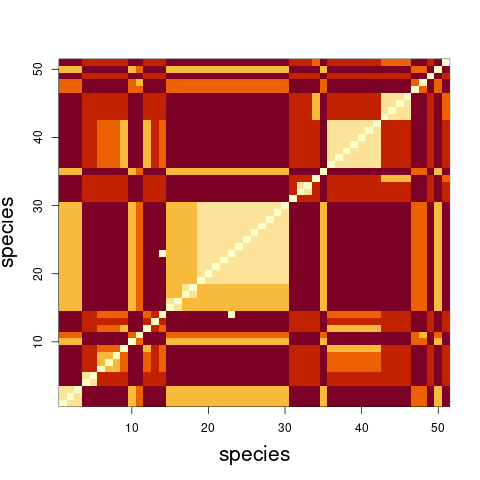
\includegraphics[width=.25\textwidth, trim=0 10 50 20, clip=]{\figbayes/FigUVSQ-Tree-GeneticDistance} &
    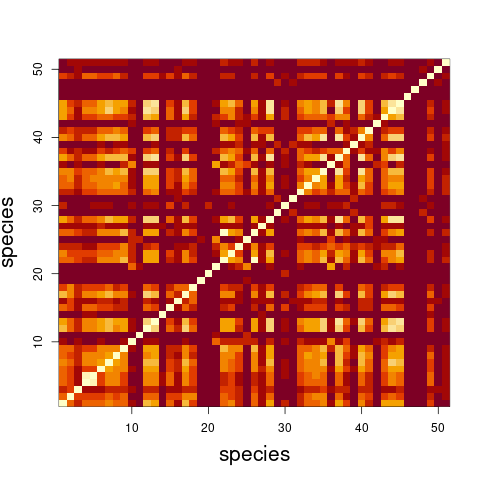
\includegraphics[width=.25\textwidth, trim=0 10 50 20, clip=]{\figbayes/FigUVSQ-Tree-GeographicDistance} & 
    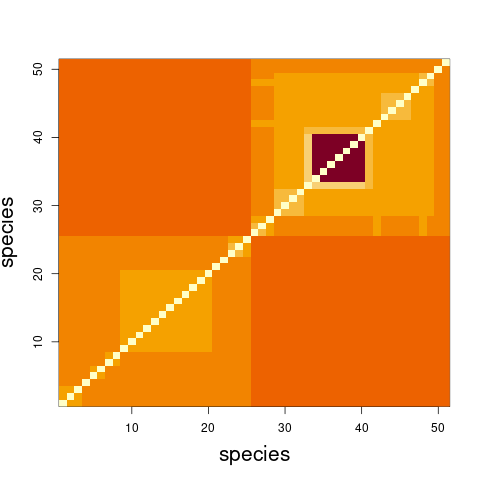
\includegraphics[width=.25\textwidth, trim=0 10 50 20, clip=]{\figbayes/FigUVSQ-Tree-TaxonomicDistance}
  \end{tabular}
  $$
  
  \pause
  \paragraph{Tree interactions.} 
  Results
  $$
  \begin{tabular}{ccc}
    Without covariate ($Q = 6$) & With covariates ($Q=4$) & Covariate effects \\
    \begin{tabular}{c}
    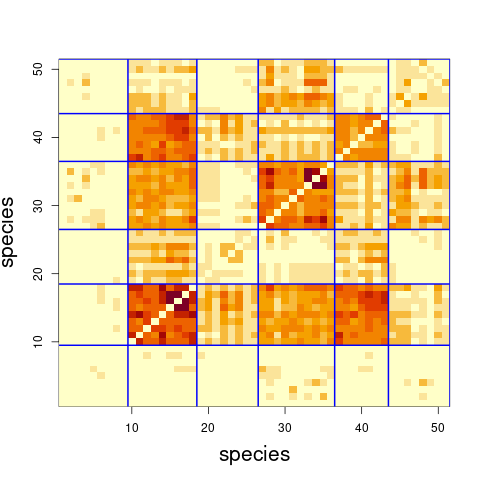
\includegraphics[width=.25\textwidth, trim=0 10 50 20, clip=]{\figbayes/FigUVSQ-Tree-ClustAdjacency-noCovar}
    \end{tabular}
    & 
    \begin{tabular}{c}
    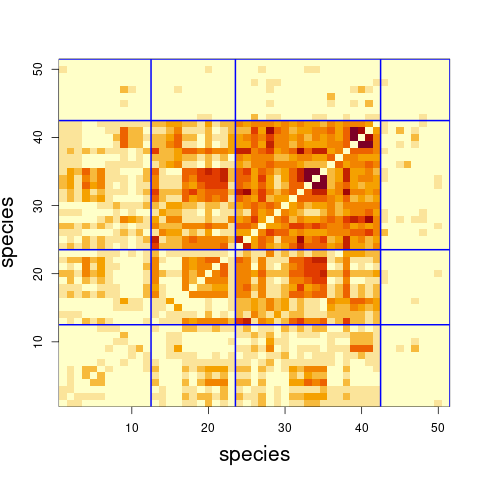
\includegraphics[width=.25\textwidth, trim=0 10 50 20, clip=]{\figbayes/FigUVSQ-Tree-ClustAdjacency-Covar}
    \end{tabular}
    &
    \begin{tabular}{l}
      $\widehat{\beta}_{\text{Gen}} = -0.413$ \\ ~ \\
      $\widehat{\beta}_{\text{Geo}} = -0.355$ \\ ~ \\
      $\widehat{\beta}_{\text{Tax}} = +0.036$
    \end{tabular}
  \end{tabular}
  $$
}

%====================================================================
%====================================================================
\section{From EM to Variationnal EM}
\frame{\frametitle{Outline} \tableofcontents[currentsection]}
%====================================================================

%====================================================================
%====================================================================
\section{Two attempts}
\frame{\frametitle{Outline} \tableofcontents[currentsection]}
%====================================================================

%====================================================================
%====================================================================
\section{Poisson log-normal model}
\frame{\frametitle{Outline} \tableofcontents[currentsection]}
%====================================================================

%====================================================================
%====================================================================
\section{Stochastic block-model}
\frame{\frametitle{Outline} \tableofcontents[currentsection]}
%====================================================================


%====================================================================
\backupbegin
%====================================================================

%====================================================================
\frame{ \frametitle{References}
{\tiny
  \nocite{DoR21}
  \bibliography{/home/robin/Biblio/BibGene}
%   \bibliographystyle{/home/robin/LATEX/Biblio/astats}
  \bibliographystyle{alpha}
  }
}

%====================================================================
\backupend
%====================================================================

%====================================================================
%====================================================================
\end{document}
%====================================================================
%====================================================================

  \begin{tabular}{cc}
    \begin{tabular}{p{.5\textwidth}}
    \end{tabular}
    &
    \begin{tabular}{p{.5\textwidth}}
    \end{tabular}
  \end{tabular}
